% \iffalse
\let\negmedspace\undefined
\let\negthickspace\undefined
\documentclass[journal,12pt,twocolumn]{IEEEtran}
\usepackage{cite}
\usepackage{amsmath,amssymb,amsfonts,amsthm}
\usepackage{algorithmic}
\usepackage{graphicx}
\usepackage{textcomp}
\usepackage{xcolor}
\usepackage{txfonts}
\usepackage{listings}
\usepackage{enumitem}
\usepackage{mathtools}
\usepackage{gensymb}
\usepackage{comment}
\usepackage[breaklinks=true]{hyperref}
\usepackage{tkz-euclide} 
\usepackage{listings}
\usepackage{gvv}  
\usepackage{tikz}
\usepackage{circuitikz} 
\usepackage{caption}
\def\inputGnumericTable{}              
\usepackage[latin1]{inputenc}          
\usepackage{color}                    
\usepackage{array}                     
\usepackage{longtable}                 
\usepackage{calc}                     \usepackage{multirow}                  
\usepackage{hhline}                    
\usepackage{ifthen}                    
\usepackage{lscape}
\usepackage{amsmath}
\newtheorem{theorem}{Theorem}[section]
\newtheorem{problem}{Problem}
\newtheorem{proposition}{Proposition}[section]
\newtheorem{lemma}{Lemma}[section]
\newtheorem{corollary}[theorem]{Corollary}
\newtheorem{example}{Example}[section]
\newtheorem{definition}[problem]{Definition}
\newcommand{\BEQA}{\begin{eqnarray}}
\newcommand{\EEQA}{\end{eqnarray}}
\newcommand{\define}{\stackrel{\triangle}{=}}
\theoremstyle{remark}
\newtheorem{rem}{Remark}

\begin{document}

\bibliographystyle{IEEEtran}
\vspace{3cm}

\title{NCERT Physics 12.7 Q21}
\author{EE23BTECH11009 - AROSHISH PRADHAN$^{*}$% <-this % stops a space
}
\maketitle
\newpage
\bigskip
\textbf{Question:} 
Obtain the resonant frequency and Q-factor of a series LCR circuit with $L = 3.0\, H$, $C = 27\, \mu F$, and $R = 7.4\, \Omega$. It is desired to improve the sharpness of the resonance of the circuit by reducing its `full width at half maximum' by a factor of 2. Suggest a suitable way.\\

\solution
Given parameters are:
\begin{table}[!h]
    \centering
    \resizebox{\columnwidth}{!}{
    \begin{table}[ht]
    \centering
    \begin{tabular}{|c|c|c|}
        \hline
        Parameter & Value & Description \\
        \hline
        $x(0)$ & 5 & First term of AP \\
        $d$ & 1.75 & Common difference of AP \\
        $x(n)$ & 20.75 & $n^{th}$ term of AP \\
        \hline
    \end{tabular}
    \vspace{2mm}
    \caption{Parameter List}
    \label{tab:simple.10.5.2.20}
\end{table}
}
    \vspace{6 pt}
    \caption{Given Parameters}
    \label{tab:1}
\end{table}
\begin{figure}[!h]
 \centering
        %\begin{circuitikz}
		% Draw the components
	%	\draw (0,0) to[V, v=$230\,V$, f=$50\,Hz$] (0,3)
	%	to[R, l=$15\,\Omega$] (3,3)
	%	to[L, l=$80\,mH$] (6,3)
	%	to[C, l=$60\,\mu F$] (6,0)
	%	-- (0,0);
    % \end{circuitikz}
\begin{circuitikz}
	\draw(0, 0) -- (1, 0);
	\draw(1, 0) to [L, l = $80\,mH$](2, 0);
	\draw(2, 0) -- (3, 0);
	\draw(3, 0) to [C, l = $60\,\mu F$](4, 0);
	\draw(4, 0) -- (5, 0);
	\draw(5, 0) to [R, l = $15\,\Omega$](6, 0);
	\draw(0, 0) -- (0, -2);
	\draw[->] (0, -1) node[left] {$I(s)$} -- (0, -1);
	\draw(6, 0) -- (7, 0);
	\draw(7, 0) -- (7, -2);
	\draw(0, -2) -- (3, -2);
	\draw(7, -2) -- (7, -2);
	\draw(3, -2) to [sV, l = $230\,V$](4, -2);
	\draw(4, -2) -- (7, -2);
\end{circuitikz}


    \caption{LCR Circuit}
    \label{fig:enter-label}
\end{figure}
\begin{enumerate}
\item {Frequency Response of the Circuit}

From Kirchhoff's Voltage Law (KVL):
\begin{equation}
V(t) = V_R + V_L + V_C \label{eq:KVL}
\end{equation}
Using reactances from \figref{fig:2},
\begin{align}
    V(s) &= R I(s) + sL I(s) + \dfrac{1}{sC} I(s)\\
    &= I(s)\left(R + Ls + \dfrac{1}{sC}\right)\\
    \implies I(s) &= \dfrac{V(s)}{\left(R + Ls + \dfrac{1}{sC}\right)} \label{eq: 4}
\end{align}
\begin{figure}[!h]
 \centering
    \begin{circuitikz}
	\draw(0,0) -- (1,0);
	\draw(1,0) to [R, l=$R$](2,0);
	\draw(2,0) -- (3,0);
	\draw(3,0) to [C, l=$\dfrac{1}{sC}$](4,0);
	\draw(4,0) -- (4,-2);
	\draw(0,-2)--(4,-2);
	\draw(0,0)--(0,-2);
	 \draw[->] (0, -1) node[left] {$I(s)$} -- (0, -1);
	 \draw(2, -2) to [sV, l =$V(s)$](2.5, -2);
\end{circuitikz}
	
    \caption{LCR Circuit}
    \label{fig:2}
\end{figure}
At resonance, the circuit becomes purely resistive. The reactances of capacitor and inductor cancel out as follows:
\begin{align}
    Ls + \dfrac{1}{sC} &= 0\\
    \implies s &= j\dfrac{1}{\sqrt{LC}} \label{eq: 6}
\end{align}
$s$ can be expressed in terms of angular resonance frequency as
\begin{equation}
    s = j\omega_0 \label{eq: 7}
\end{equation}
Comparing \eqref{eq: 6} and \eqref{eq: 7}, we get
\begin{equation}
    \omega_0 = \dfrac{1}{\sqrt{LC}}
\end{equation}
\item{Quality Factor}

\begin{enumerate}
\item Using voltage across inductor,
\begin{align}
    Q &= \left(\dfrac{V_L}{V_R}\right)_{\omega_0} = \dfrac{\lvert{sLI(s)}\rvert}{\lvert RI(s) \rvert}\\
    &= \dfrac{1}{\sqrt{LC}}\dfrac{L}{R}\\
    &= \dfrac{1}{R}\sqrt{\dfrac{L}{C}}
\end{align}
\item Using voltage across capacitor,
\begin{align}
	Q &= \left(\dfrac{V_C}{V_R}\right)_{\omega_0} = \dfrac{\abs{\frac{I(s)}{sC}}}{\lvert RI(s) \rvert}\\
    &= \dfrac{\sqrt{LC}}{RC}\\
    &= \dfrac{1}{R}\sqrt{\dfrac{L}{C}}
\end{align}
\end{enumerate}
\item{Plot of Impedance vs Angular Frequency}

Impedance is defined as
\begin{equation}
    H(s) = \dfrac{V(s)}{I(s)}
\end{equation}
Using \eqref{eq: 4},
\begin{align}
     H(s) &= R + sL + \dfrac{1}{sC}\\
     \implies H(j\omega) &= R + j\omega L + \dfrac{1}{j\omega C}\\
     \implies \lvert H(j\omega) \rvert &= \sqrt{R^2 + \left(\omega L - \dfrac{1}{\omega C}\right)^2}
\end{align}
\begin{figure}[!h]
    \centering
    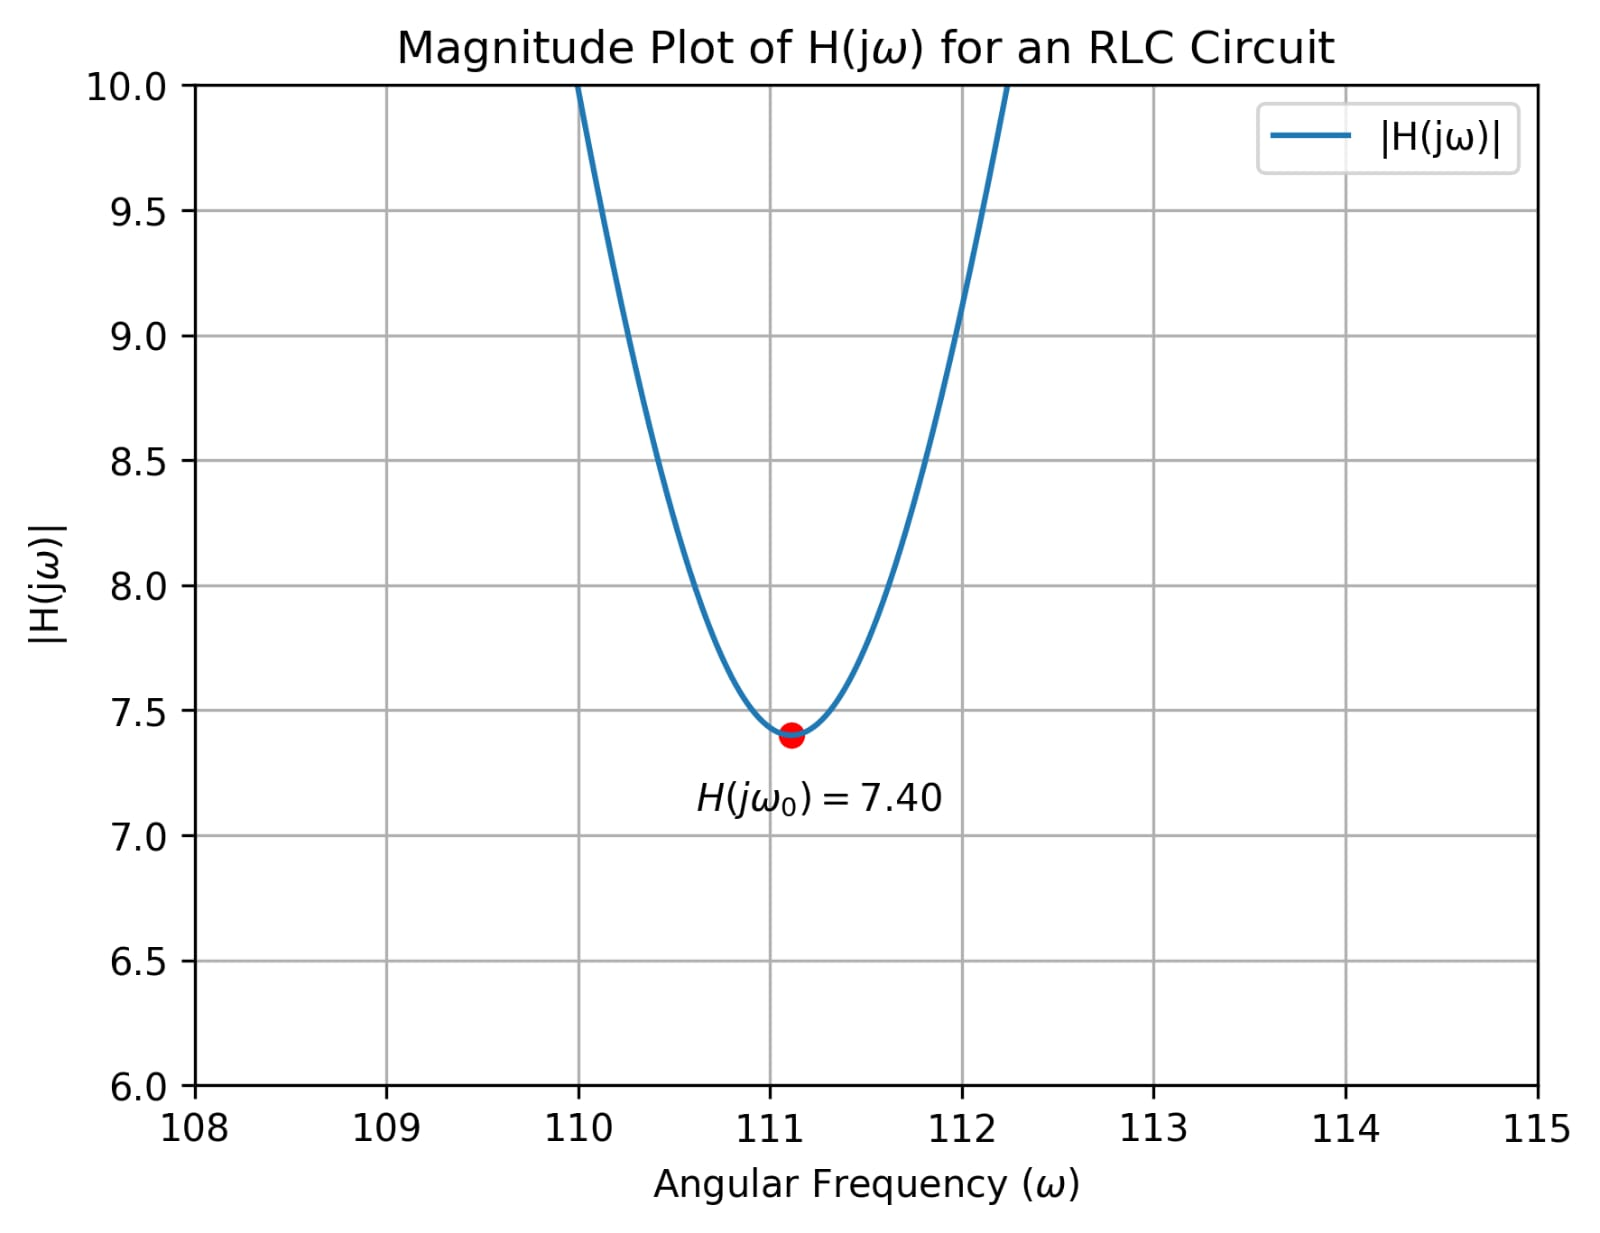
\includegraphics[width = \columnwidth]{figs/h_plot.png}
    \caption{Impedance vs $\omega$ (using values in \tabref{tab:1})}
    \label{fig:h_plot}
\end{figure}
\end{enumerate}
\end{document}
